%% 
%% Copyright 2007, 2008, 2009 Elsevier Ltd
%% 
%% This file is part of the 'Elsarticle Bundle'.
%% ---------------------------------------------
%% 
%% It may be distributed under the conditions of the LaTeX Project Public
%% License, either version 1.2 of this license or (at your option) any
%% later version.  The latest version of this license is in
%%    http://www.latex-project.org/lppl.txt
%% and version 1.2 or later is part of all distributions of LaTeX
%% version 1999/12/01 or later.
%% 
%% The list of all files belonging to the 'Elsarticle Bundle' is
%% given in the file `manifest.txt'.
%% 

%% Template article for Elsevier's document class `elsarticle'
%% with numbered style bibliographic references
%% SP 2008/03/01

\documentclass[preprint,12pt, a4paper]{elsarticle}

%% Use the option review to obtain double line spacing
%% \documentclass[authoryear,preprint,review,12pt]{elsarticle}

%% For including figures, graphicx.sty has been loaded in
%% elsarticle.cls. If you prefer to use the old commands
%% please give \usepackage{epsfig}

%% The amssymb package provides various useful mathematical symbols
\usepackage{amssymb}
\usepackage{amsmath}
%% The amsthm package provides extended theorem environments
%% \usepackage{amsthm}

%% The lineno packages adds line numbers. Start line numbering with
%% \begin{linenumbers}, end it with \end{linenumbers}. Or switch it on
%% for the whole article with \linenumbers.
\usepackage{lineno}

\usepackage{float}
\restylefloat{table}

\usepackage{hyperref}

\journal{SoftwareX}

\begin{document}

%%%%%%%%%%%%%%%%%%%%%%%%%%%%%%%%%%%%%%%%%%%%%%%%%%%%%%%%%%%%%%%%%%%%%%%%%%%%%%%
\begin{frontmatter}

%% Title, authors and addresses

%% use the tnoteref command within \title for footnotes;
%% use the tnotetext command for theassociated footnote;
%% use the fnref command within \author or \address for footnotes;
%% use the fntext command for theassociated footnote;
%% use the corref command within \author for corresponding author footnotes;
%% use the cortext command for theassociated footnote;
%% use the ead command for the email address,
%% and the form \ead[url] for the home page:
%% \title{Title\tnoteref{label1}}
%% \tnotetext[label1]{}
%% \author{Name\corref{cor1}\fnref{label2}}
%% \ead{email address}
%% \ead[url]{home page}
%% \fntext[label2]{}
%% \cortext[cor1]{}
%% \address{Address\fnref{label3}}
%% \fntext[label3]{}

\title{One-dimensional turbulence (ODT): computationally efficient modeling and simulation of turbulent  flows}

%% use optional labels to link authors explicitly to addresses:
%% \author[label1,label2]{}
%% \address[label1]{}
%% \address[label2]{}

%\renewcommand{\thefootnote}{\fnsymbol{footnote}}
\author{Victoria B. Stephens}
\author{David O. Lignell\corref{cor1}}

\cortext[cor1]{Corresponding author. \ead{davidlignell@byu.edu}}

\address{Chemical Engineering Department, Brigham Young University, Provo, UT 84602, USA}

\begin{abstract}
Write this last. About 100 words. 
\end{abstract}

\begin{keyword}
%% keywords here, in the form: keyword \sep keyword
turbulence \sep reacting flows \sep one-dimensional turbulence

%% PACS codes here, in the form: \PACS code \sep code

%% MSC codes here, in the form: \MSC code \sep code
%% or \MSC[2008] code \sep code (2000 is the default)

\end{keyword}

\end{frontmatter}

%%%%%%%%%%%%%%%%%%%%%%%%%%%%%%%%%%%%%%%%%%%%%%%%%%%%%%%%%%%%%%%%%%%%%%%%%%%%%%%
\section*{Code Metadata}
\label{metadata}

\begin{table}[H]
\begin{tabular}{|l|p{6.5cm}|p{6.5cm}|}
\hline
\textbf{Nr.} & \textbf{Code metadata description} & \textbf{Please fill in this column} \\
\hline
C1 & Current code version & 1.0 \\
\hline
C2 & Permanent link to code/repository used for this code version & \href{https://github.com/BYUignite/ODT}{https://github.com/BYUignite/ODT} \\
\hline
C3 & Code Ocean compute capsule & N/A\\
\hline
C4 & Legal Code License   & MIT \\
\hline
C5 & Code versioning system used & Git \\
\hline
C6 & Software code languages, tools, and services used & C++, Python 3.x, Yaml,  \\
\hline
C7 & Compilation requirements, operating environments \& dependencies & CMake 3.12+, Cantera, Git, Doxygen (optional) \\
\hline
C8 & If available Link to developer documentation/manual & \href{https://byuignite.github.io/ODT/doxygen/html/style_guide.html}{style guide} \\
\hline
C9 & Support email for questions & davidlignell@byu.edu \\
\hline
\end{tabular}
\caption{Code metadata (mandatory)}
\end{table}


\linenumbers

%The permanent link to code/repository or the zip archive should include the following requirements: 
%\begin{itemize}
%	\item README.txt and LICENSE.txt.
%	\item Source code in a src/ directory, not the root of the repository.
%	\item TO DO: Tag corresponding with the version of the software that is reviewed.
%	\item TO DO: Documentation in the repository in a docs/ directory, and/or READMEs, as appropriate.
%\end{itemize}

%%%%%%%%%%%%%%%%%%%%%%%%%%%%%%%%%%%%%%%%%%%%%%%%%%%%%%%%%%%%%%%%%%%%%%%%%%%%%%%
\section{Motivation and significance}
\label{sec:motivation}

Turbulent flows characterize the vast majority of fluid flows in practical engineering applications, and simulations of turbulent flows provide researchers with valuable insights into complex systems, particularly reacting turbulent flows such as combustion processes. Turbulence is a complex phemonenon that affects the full range of a flow's length and time scales. As a result, resolving the entire flow field by numerically solving the Navier-Stokes equations of fluid flow, as is done in direct numerical simulations (DNS), requires substantial computational resources. DNS is a powerful research tool, but its high computational cost makes it intractable for simulating most practical engineering flows. In order to achieve numerical solutions to practical flow problems, researchers can use alternative frameworks that model turbulence rather than resolving it directly.

Large-eddy simulations (LES) address the problem of wide-ranging length and time scales by combining  direct resolution of grid-scale quantities, as in DNS, with subgrid modeling of smaller turbulence structures. The more complex the flow, the more modeling is required; for example, a jet flame simulation might require subgrid modeling for the combustion chemistry, radiative heat transfer, or soot chemistry in addition to turbulence structures, all of which form a tightly coupled system in which each model interacts heavily with the others. While subgrid modeling makes LES more computationally affordable than DNS, it can introduce empiricism into simulations, which can lead to inaccurate results. Additionally, unresolved quantities are often parameterized in state space with empirical relationships or assumed distributions that lack universal applicability. LES is a valuable simulation tool, but its approach to turbulence modeling can introduce unwanted empiricism and make errors difficult to isolate and quantify.

The one-dimensional turbulence model (ODT) functionally reverses the LES approach, modeling large-scale turbulent advection and directly resolving small-scale flow structures, simulating the full range of length and time scales in a single dimension. Depending on the configuration, large-scale structures can be easier to model than small-scale structures (especially when reaction is present. ODT's direct resolution (in one dimension) of fine scales removes subgrid modeling issues that complicate LES. Previous studies show that ODT can attain accuracy comparable to DNS at a fraction of the computational cost \cite{Lignell_2015,Abboud_2015}, making it an attractive tool for simulating turbulent flows. Because the ODT model is one-dimensional, it is limited to homogeneous or boundary-layer flows, such as jets, wakes, and mixing layers; these types of flows, however, are common in nature and central to turbulence research. ODT's computational efficiency and resolution of a full range of scales make it a valuable tool that complements experimental studies and other simulation tools like DNS and LES. 

Early applications of ODT focused on homogenous turbulence, wakes, and mixing layers \cite{Kerstein_1999,Kerstein_2000,Kerstein_2001}. Later extension to variable-density flows and a spatial downstream coordinate system facilitated its growth and application to more complex flows, including combustion in jet flames \cite{Echekki_2001,Hewson_2001,Hewson_2002,Lignell_2012,Punati_2011,Abdelsamie_2017,Lignell_2017, Goshayeshi_2015}, counterflow flames \cite{Jozefik_2015}, wall fires \cite{Monson_2016}, and sooting flames \cite{Lignell_2015,Hewson_2006,Hewson_2009,Lignell_2015b,Ricks_2010}, as well as other particle flows \cite{Sun_2017,Schmidt_2009,Sun_2014,Fistler_2017}. ODT has also served to complement LES through subgrid modeling studies \cite{Cao_2008,Schmidt_2003,Schmidt_2010} and has been applied to various other flow configurations such as double-diffusive interfaces \cite{GonzalezJuez_2011}, Rayleigh-Taylor mixing \cite{GonzalezJuez_2013}, and stratified turbulence \cite{Wunsch_2001}. Most recently, the ODT code was extended to include cylindrical and spherical coordinate systems \cite{Lignell_2018,Klein_2018,Klein_2019}.

During the recent implementation of the cylindrical and spherical model formulations, the ODT code was drastically overhauled and reorganized, resulting in its current configuration. The ODT code presented here is a pared down version of the development code, representing the fundamental aspects of the ODT model and its most reliable functions. The example cases in Section~\ref{sec:examples} are a representative sample of the ODT code's capabilities as it is presented here. Future releases will expand this code's functionality with additional features currently in development. 

%Questions to answer in this section (from SoftwareX template)
%\begin{enumerate}
%	\item What's the scientific background and motivation for this software?
%	\item Why is this important? What problems does it solve?
%	\item How has the software contributed (and/or how will it contribute in the future) to the process of scientific discovery? Cite papers using the software.
%	\item In what experimental setting might someone use this software?
%	\item What related work is there in the literature?
%	\item What algorithms, other code/software, or ideas are used? Cite them. 
%\end{enumerate}

%%%%%%%%%%%%%%%%%%%%%%%%%%%%%%%%%%%%%%%%%%%%%%%%%%%%%%%%%%%%%%%%%%%%%%%%%%%%%%%
\section{Software description}
\label{sec:description}

\subsection{Model description}
\label{sub:model_description}

The ODT model is described in detail in the literature~\cite{Kerstein_1999,Kerstein_2001,Ashurst_2005,Lignell_2018,Lignell_2013}; only a brief explanation will be given here. In ODT, turbulent advection is modeled with stochastic processes called eddy events, which punctuate the solution of unsteady, one-dimensional transport equations for mass, momentum, and enthalpy. The ODT code uses a Lagrangian finite-volume formulation for diffusive advancement in which mass stays constant within each grid cell while cell volumes increase or decrease according to cell dilation via an adaptive mesh refinement~\cite{Lignell_2013}.

Transport equations for mass, momentum, and enthalpy in the temporal formulation of ODT take the following generic form, derived from the Reynolds Transport Theorem~\cite{Cengel_2010} for a given scalar quantity per unit mass $\beta$: 
\begin{equation} 
\label{eq:transport}
	\frac{\mathrm{d}\beta}{\mathrm{d}t} = -\frac{j_{\beta,e}A_{x,e}-j_{\beta,w}A_{x,w}}{\rho V} + \frac{S_{\beta}}{\rho V}.
\end{equation}
Here, $j_{\beta}$ is the diffusion flux of scalar $\beta$ across the cell face area $A_x$ where the subscripts $e$ and $w$ refer to the ``east" and ``west" faces of a given grid cell, respectively. $S_{\beta}$ is the Lagrangian source term derived from the conservation law for $\beta$, $\rho$ represents mass density, and $V$ represents cell volume. In practice, we refer to the left hand term on the right side of Equation~\ref{eq:transport} as the ``mixing term" and the right hand term on the right side of Equation~\ref{eq:transport} as the ``source term". The generic transport equation differs slightly in the spatial formulation of ODT, but its form is similar, so we omit it here for brevity. The system of ordinary differential equations (ODEs) that results is well behaved at all grid points and in all geometries in their finite-volume forms. For details on transport equation derivation and use in both the temporal and spatial formulations of ODT, see Lignell et al.~\cite{Lignell_2018}. 

Eddy events occur as a Poisson process in accordance with their eddy rates, where a given eddy event of size $l$ and location $x_0$ has an eddy timescale $t$ and an associated eddy rate $1/t$. Three user-defined ODT parameters control the eddy event process: the eddy rate parameter $C$ scales the rate of occurrence of the eddies; the viscous penalty parameter $Z$ suppresses small eddies; and the large eddy suppression parameter $\beta_{LES}$ constrains eddies to those with timescales proportional to the elapsed simulation time. Sampled eddies that do not fit the defined parameters are rejected and not applied to the domain.

Eddy events modify domain variables using ``triplet maps", as illustrated in Figure~\ref{fig:tripletmap}. In an eddy region of size $l$, transported property profiles are modified (mapped) by making three copies, compressing each spatially by a factor of three, then lining these up with the middle copy spatially reversed.
This map is continuous and conservers all quantities and statistical moments, increases scalar gradients and decreases length scales consistent with turbulent eddies in real flows. Subsequent eddies in the same region will result in a cascade of scales. The eddy rates, used in the sampling and selection of eddies depend on eddy size and the local kinetic energy consistent with turbulent scaling laws.  

\begin{figure}
	\centering
	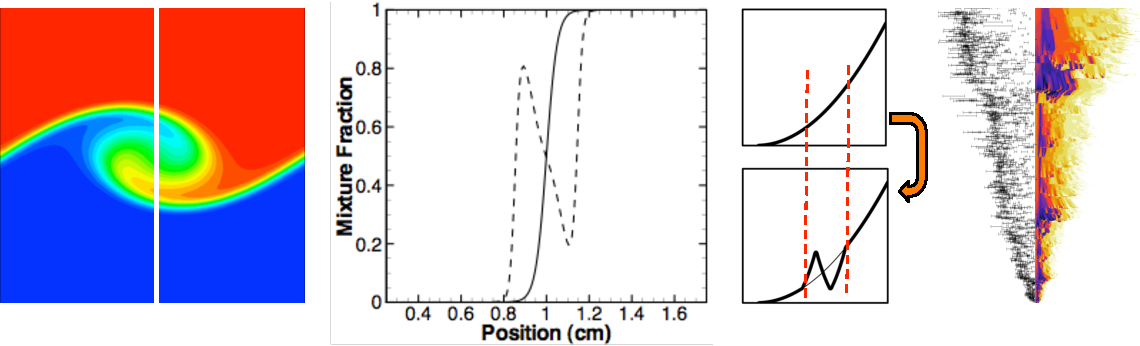
\includegraphics[width=\textwidth]{../figures/tripletmap/tripmap.pdf} 
    \caption{Schematic diagram of a triplet map. From left to right: (first pane) simulation of a single ``eddy", a two-dimensional Kelvin-Helmholz instability with a vertical white line-of-sight; (second pane) mixture fraction profile along the indicated line-of-sight before and after the eddy showing increased gradients and surface area; (third pane) a triplet map operates on a profile to produce a mapped profile with three copies, compressed and lined up, with the middle copy spatially inverted; (fourth pane) illustrative eddy event sizes and locations with corresponding temperature profile for a single ODT realization of a wall fire, adapted from \cite{Monson_2016}.}
	\label{fig:tripletmap}
\end{figure}

Eddy events occur concurrently with diffusive advancement via solution of the system of unsteady one-dimensional transport equations. In this way, the ODT code marches in time (or space) until it reaches its end point. Due to the stochastic nature of eddy events, each ODT simulation, or realization, is different, even when it is provided with the same input parameters. In order to obtain statistically stable data for a given set of parameters, we run many realizations with the same input parameters, and then gather statistics over these realizations. This is done via post-processing tools, which are provided in the ODT package. 

%-----------------------------------------------------------------------------------
\subsection{Software Architecture}
\label{sub:architecture}

The ODT package consists primarily of an object-oriented C++ code responsible for running flow simulation cases and generating data. The package also contains auxiliary data processing and visualization tools, written mostly in Python. The post-processing tools are case-specific but will be  addressed generally in Section~\ref{sub:workflow}. 

\begin{figure}
	\centering
	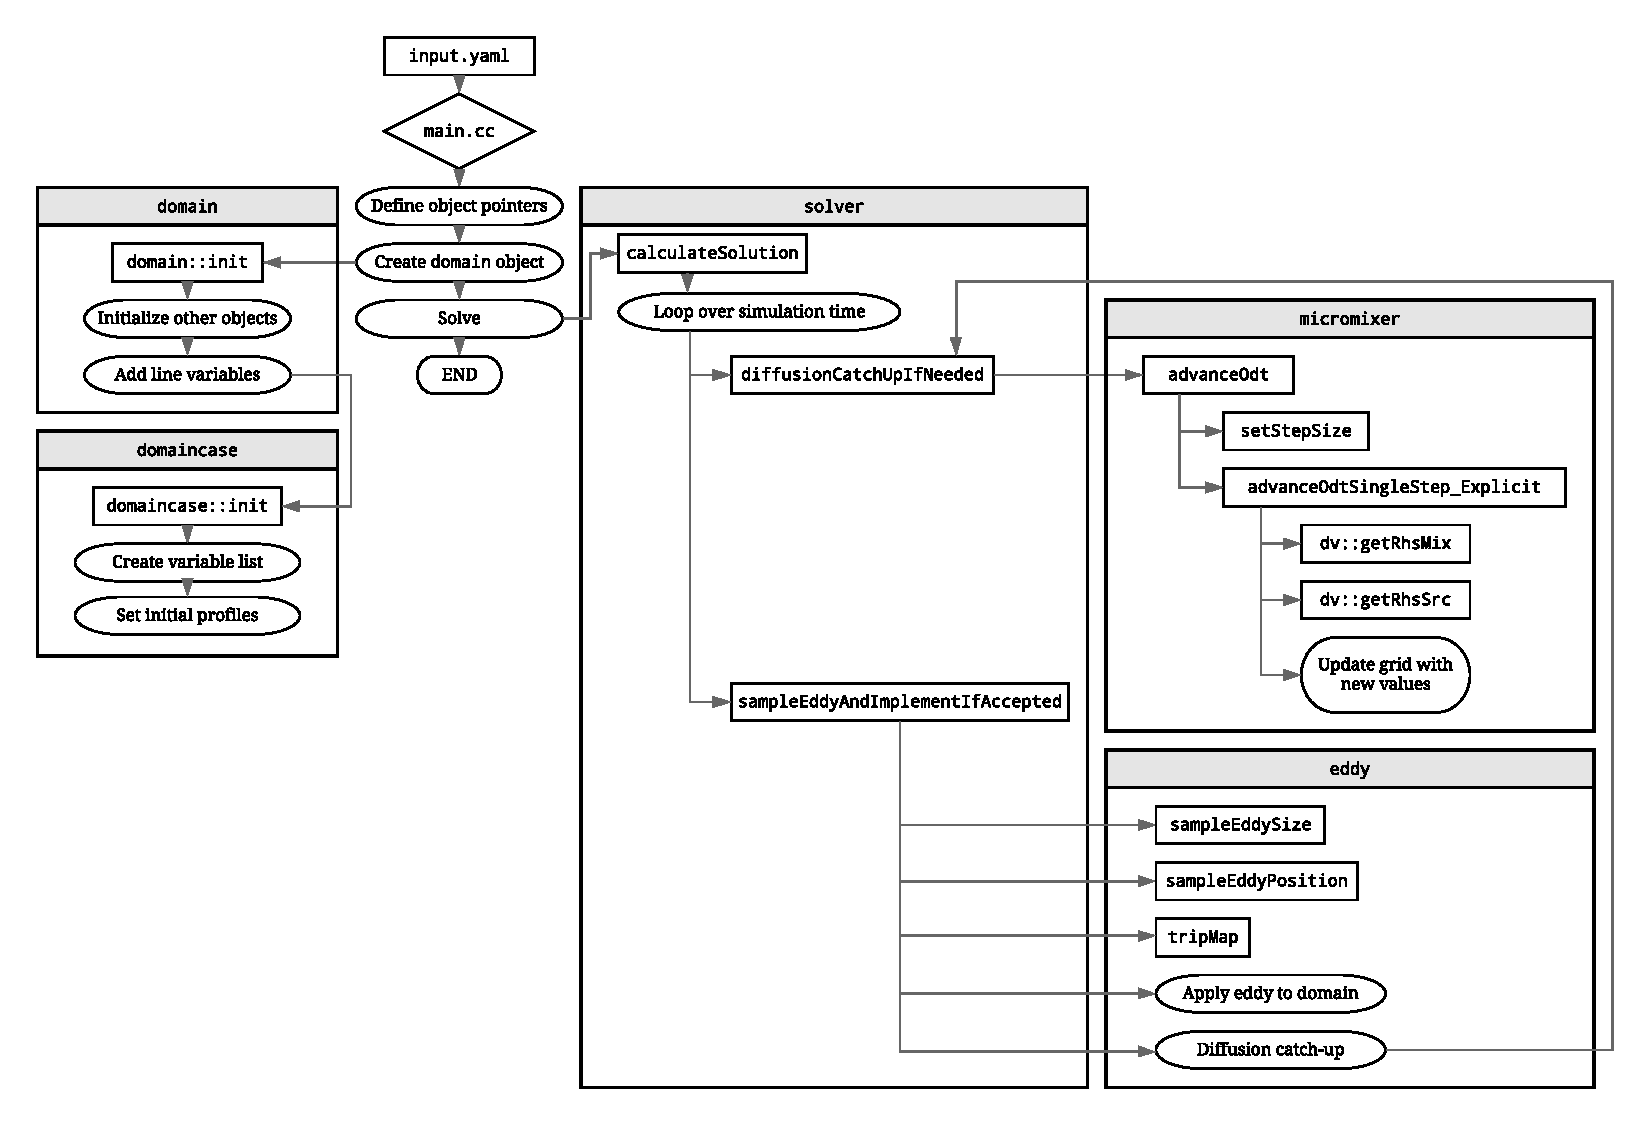
\includegraphics[width=\textwidth]{../figures/odt_flow_chart.pdf} 
	\caption{Structural outline of the ODT code, including its major class objects. For brevity, this diagram makes two simplifications. First, it assumes that diffusive advancement in the \texttt{micromixer} uses an explicit solution method; in practice, users specify either an explicit, semi-implicit, or Strang split method. Second, it implies that all of the eddy events sampled by the \texttt{eddy} object are applied to the domain; in reality, eddy events are filtered through several rejection tests (omitted from this figure for clarity) before acceptance and application to the domain.}
	\label{fig:flowchart}
\end{figure}

Figure~\ref{fig:flowchart} illustrates the ODT code's most important objects and structural features. User inputs are provided to the executable in YAML \cite{Beder_2008} format via \texttt{input.yaml}; the location of the specific \texttt{input.yaml} file to be used is determined by the case name and case type specified in the run script. The \texttt{main} function defines storage for the main objects, but, once created, the \texttt{domain} object is responsible for object initialization as well as variable initialization and storage via a case-specific \texttt{domaincase} object. 

Three primary objects handle the code's main functions: the \texttt{solver}, \texttt{micromixer}, and \texttt{eddy} objects. The \texttt{solver} coordinates the ODT solution process, marching along the simulation time and invoking diffusive advancement and eddy events. The \texttt{micromixer} handles diffusive advancement by setting step sizes, interacting with the transported domain variables, and solving the system of ODEs defined by Equation~\ref{eq:transport} (or its equivalent in the spatial formulation). The \texttt{micromixer} includes three solution methods that can be specified in \texttt{input.yaml}: a first-order explicit Euler method (pictured in Figure~\ref{fig:flowchart}); a first-order semi-implicit method; and a second order Strang splitting method~\cite{Strang_1968}. The latter two methods are useful for treating stiff chemistry, with source terms integrated using CVODE~\cite{Hindmarsh_2020}.
In reacting flow cases, enthalpy and chemisal species are transported, with physical properties and kinetic rates computed with Cantera~\cite{Goodwin_2018}. The \texttt{micromixer} is also the code's primary point of interaction with the \texttt{mesher} object (not pictured in Figure~\ref{fig:flowchart}), which manages the adaptive grid functions. Finally, the \texttt{eddy} object manages eddy event selection and implementation, which proceeds as described in Section~\ref{sub:model_description}.  

%Things to put in this section (from SoftwareX template)
%\begin{itemize}
%	\item overview of overall software architecture
%	\item optional: pictorial overview
%	\item implementation details
%\end{itemize}

%-----------------------------------------------------------------------------------
\subsection{Workflow}
\label{sub:workflow}

This section outlines the process a user goes through in order to successfully build the ODT code and run a simulation. For more details, please see the package documentation. ODT is a standalone, self-contained package, and users interact with its files primarily via the command line rather than a graphical interface. 

Within the main download package, several directories organize the ODT code. The \texttt{source}, \texttt{build}, and \texttt{run} directories contain the ODT source code, compilation tools, and run scripts, respectively. The \texttt{input} directory contains subdirectories corresponding to several possible case types, each populated with an appropriate input files. The \texttt{data} directory, initially empty, holds the raw data files and runtime information generated by ODT, as well as post-processed data files generated from within the \texttt{post} directory. Finally, the \texttt{doc} directory contains documentation optionally generated by Doxygen \cite{vanHeesch_2018} during the build process. 

\subsubsection{Building ODT}

The ODT build process is automated with CMake. The user navigates to the \texttt{build} directory and edits the CMake configuration file. The CMake configuration file specifies Cantera's location and must be changed to reflect the local installation location. For reacting flows, the chemical reation rates can be computed by Cantera (the default), or a from a user-specified function, specified at compile time. Once the configuration settings are updated, the user runs CMake to apply the changes. 

YAML is required in order to process input files. If it has not yet been installed, it must be built and installed at this point. For convenience, the ODT package automates this process. YAML need only be installed once for a given instance of the ODT package. Rebuilding the ODT code with CMake does not affect the YAML installation. 

Once CMake and YAML have been prepared, the user can build the ODT code with the \texttt{make} command, which places the code executable in the \texttt{run} directory. The most common errors that occur during the build process involve incorrect file paths or incomplete installation of required packages. See the build documentation for troubleshooting help. 

Once the code is built, the user may optionally build a local copy of the documentation via Doxygen, which must be previously installed. This step is not required in order to run the ODT code. As an alternative, documentation can be accessed at the code repository wiki. 

\subsubsection{Input files}

User-modified input files are located within the \texttt{input} directory, which contains subdirectories that correspond to various case types that can be run with ODT. At minimum, a case's subdirectory must contain an \texttt{input.yaml} file, but may contain other files, or subfolders with supplementary information. 
%ODT has the capability to restart a simulation from a specified time or state. To use this function, a raw data file at the required state must be copied to the input case directory and renamed \texttt{restart.dat}. For an example, please see the \texttt{jetFlame/flameD} case. Note that the user must also change the \texttt{Lrestart} parameter within the \texttt{input.yaml} file in order to use the restart feature. 

The \texttt{input} directory also contains the \texttt{gas\textunderscore mechanisms} subdirectory, which contains chemical mechanism files that can be used in reacting flow cases. For cases in which a chemical mechanism is not required, the \texttt{not\textunderscore used.xml} mechanism file is specified in \texttt{input.yaml}. Note that the chemical mechanism chosen for the case and specified in the input file must match the mechanism specified in the CMake configuration file during the ODT build process. 

Input files contain simulation parameters in a human-readable format parsed by YAML. Details about individual parameters, including usage and typical values, are covered in the documentation. Within \texttt{input.yaml}, parameters are organized into sections, several of which are common to all input files. Parameter values present in the provided input files may be considered defaults that may be used to run a successful simulation of that case type. General code parameters are stored in the \texttt{params} class. Variables needed in a simulation but not provided in an input file (not recommended), are either given defaults specified in the \texttt{params} class, or result in an error message. 

%An overview of possible ODT parameters will be covered here, but does not represent all the possibilities or functions of ODT; please see the associated documentation for more information. Input files are divided into sections, several of which are common to all \texttt{input.yaml} files; these are summarized in Table \ref{tab:input_sections}. 

%\begin{table}
%\begin{tabular}{|l|p{4.1in}|}
%\hline
%Section 				& Description 	\\
%\hline
%\texttt{params}* 		& General parameters, including simulation length, domain size, and ODT parameters ($C$, $Z$, $\beta_{LES}$) \\
%\texttt{radParams}		& Radiation parameters; only relevant to reacting flow cases (i.e. jet flames) \\
%\texttt{streamProps}	& Stream properties; used when there are two or more separate streams (i.e. non-premixed jets)\\
%\texttt{bcCond}* 		& Boundary conditions for velocity and temperature (where required) \\
%\texttt{initParams} 	& Case-specific initialization parameters, usually flow geometry and stream velocities \\
%\texttt{dumpTimes}*		& List of simulation time steps at which to output data files \\
%\hline
%\end{tabular}
%\caption{Common sections present in \texttt{input.yaml} files. Sections marked with a * should be present in every \texttt{input.yaml} file regardless of case type. Sections usually appear in this order, but this is not required.}
%\label{tab:input_sections}
%\end{table}

\subsubsection{Running ODT}

To run a simulation, users must then navigate to the \texttt{run} directory, which contains the \texttt{odt.x} executable and several possible run scripts. The simplest option is \texttt{runOneRlz.sh}, which runs one realization of ODT in the specified configuration. In this run script, the user must alter two variables near the top of the file: \texttt{inputDir}, which specifies which input directory and files to use; and \texttt{caseName}, which provides a name for the simulation and the data files it outputs. The \texttt{runManyRlz.sh} script runs many realizations in serial, one after the other; it differs from \texttt{runOneRlz.sh} only in that the user must also alter the \texttt{nRlz} variable, which specifies the number of realizations to run. Realizations differ by having different random seeds (specified in the input file). The random seed can either be randomized, or directly specified. To run the simulation with either \texttt{runOneRlz.sh} or \texttt{runManyRlz.sh}, save the run script and execute it at the command line. Users will see some output on the command line, but no data, which is instead output to the \texttt{data} directory.  

ODT simulations can also be run in parallel using MPI. Two run scripts, \texttt{slrmJob.sh} and \texttt{slrmJob\textunderscore array.sh}, are configured using SLURM \cite{Yoo_2003}, a common workload manager used for massively parallel computing resources. This allows many ODT realizations to run in parallel rather than in serial, reducing overall simulation time. Individual realizations are independent (\emph{embarrassingly parallel}), but users must take care with case names and input file changes to ensure that individual realizations or entire cases are not overridden accidentally. 

\subsubsection{Data files and post-processing}

For a given simulation, data is output to the \texttt{data} directory, which contains subdirectories for each simulation, specified by the \texttt{caseName} variable in the run script. Figure \ref{fig:data_folder_structure} illustrates the structure of the \texttt{data} directory and the locations of files within it. Each case folder is subdivided into \texttt{input}, \texttt{runtime}, \texttt{data}, and \texttt{post}. The \texttt{input} folder contains a copy of the input files used for the simulation; \texttt{runtime} contains runtime output information, such as eddy event information ; \texttt{data} contains the raw data files; and \texttt{post} contains post-processed data files once they are generated. 

\begin{figure}
	\centering
	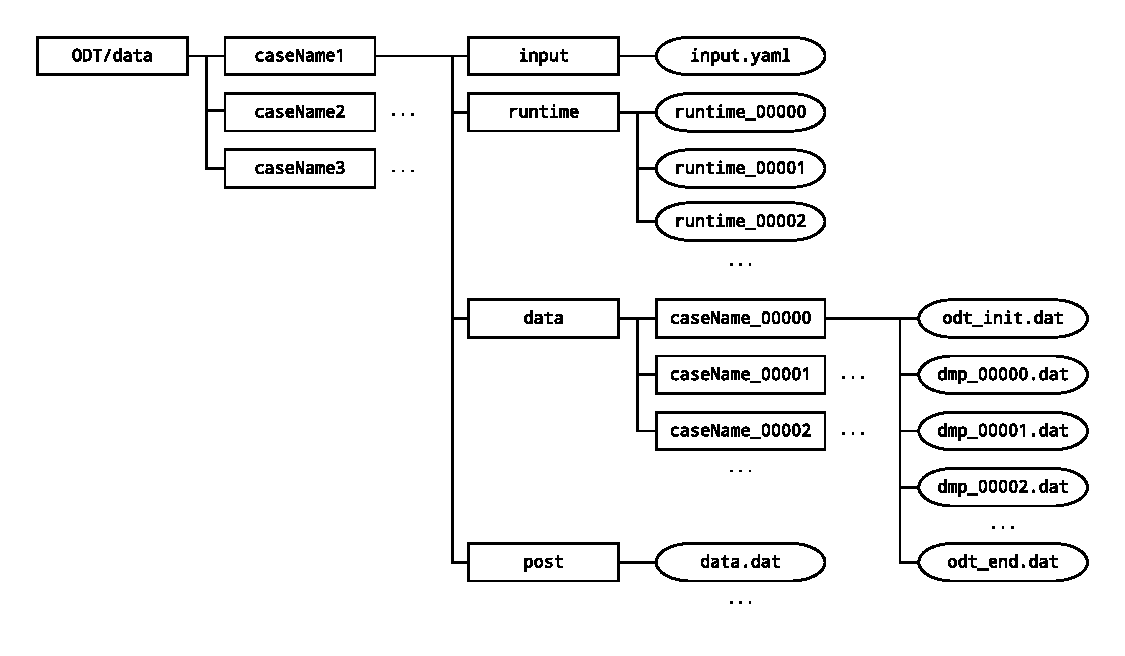
\includegraphics[width=\textwidth]{../figures/data_folder_structure.pdf} 
	\caption{Data folder structure and file locations. Boxes indicate folders and ovals indicate files. For a given simulation, \texttt{caseName} will be replaced with the case name specified in the run script. The number attached to \texttt{caseName} folder names and to \texttt{runtime} data files indicates the realization number. The number attached to \texttt{dmp} files indicates the output time step, or ``dump" time, of the data file. These correspond to the order of the time steps listed in \texttt{input.yaml}.}
	\label{fig:data_folder_structure}
\end{figure}

To use post-processing tools, navigate to the \texttt{post} directory. Within the \texttt{post} directory, data processing tools are organized by case type, which is specified in \texttt{input.yaml} and determines case-specific variables and simulation setup parameters (refer to the \texttt{domaincase} object in Figure \ref{fig:flowchart}). Each set of post-processing tools is different, but may contain some combination of Python scripts (often coordinated by a \texttt{driver.py} file), experimental data files for comparison and plot generation, or other supplementary files. Post-processed data and generated plots are deposited in the \texttt{data} directory, within the appropriate \texttt{caseName/post} folder. 
%For more information on using the provided post-processing tools, please refer to the documentation. 

% reference video that we will eventually make?

%%%%%%%%%%%%%%%%%%%%%%%%%%%%%%%%%%%%%%%%%%%%%%%%%%%%%%%%%%%%%%%%%%%%%%%%%%%%%%%
\section{Example Case: Canonical Jet Flame}
\label{sec:examples}

%%-----------------------------------------------------------------------------------
%\subsection{Pipe Flow}
%\label{sub:pipeflow}
%
%% TEXT COPIED/MODIFIED FROM CYLINDRICAL ODT PAPER
%First, we present an incompressible pipe flow simulation using the temporal, cylindrical ODT formulation. Results for three different friction Reynolds numbers ($Re_\tau$ = 550, 1000, 2000) are compared to DNS results from El Khoury et al. \cite{ElKhoury_2013} ($Re_\tau$ = 550, 1000) and Chin et al. \cite{Chin_2014} ($Re_\tau$ = 2000) for a pipe diameter of $D=2.0$ m and flow density of 1.0 kg$\cdot$m$^{-3}$. Friction velocity values of 1 m$\cdot$s$^{-1}$ ($Re_\tau = 550, 1000$) and 2 m$\cdot$s$^{-1}$ ($Re_\tau = 2000$) were assumed and used to calculate the mean pressure gradient driving the flow. Using initial conditions with uniform velocity profiles, simulations were run until a state of developed flow was achieved, at which point data were gathered until statistical convergence for the root mean square (RMS) velocity difference from the mean profiles occurred. 
%
%The simulations were performed with ODT parameters $C = 5$ and $Z = 350$ for the temporal ODT formulation. 
%%Additionally, a restriction was imposed on the eddy size range by selecting eddies only up to a maximum normalized size of Le,max/D = 1/3. This restriction limits the eddy size by construction, as opposed to the large-eddy suppression mechanism commonly used in ODT simulations [27,45]. 
%The values of C and Z
%%and Le,max/D 
%were adjusted to give good agreement of the ODT results compared to the DNS. Schmidt et al. \cite{Schmidt_2003} showed that higher $Z$ results in the buffer-layer being located further from the wall, and increasing $C$ results in a lower slope of the mean streamwise velocity in the log-layer.
%%and higher Le,max/D gives a smaller mean streamwise velocity in the wake region.
%
%RESULTS AND PLOTS GO HERE
%
%\subsection{Non-reacting Jet }
%\label{sub:nonreactingjet}
%
%% TEXT COPIED/MODIFIED FROM CYLINDRICAL ODT PAPER
%Here, we present ODT simulation results for a non-reacting round, turbulent jet compared to the experimental data of Hussein et al. \cite{Hussein_1994}. The jet consists of air issuing into air through a 1 in (0.0254 m) diameter duct with a uniform exit velocity of 56.2 m$\cdot$s$^{-1}$ and a reported Reynolds number of 95,500. The ODT simulations use this diameter and velocity with a kinematic viscosity of $1.534\cdot10^{-5}$ m$^2$s$^{-1}$, resulting in a Reynolds number of 93,056. The initial velocity profile in the ODT simulations is a modified top-hat profile in which a hyperbolic tangent function of width $\delta$ = 0.1D is used on either side of the jet to smooth the transition between the jet and the free stream. In the spatial formulation of ODT, the streamwise velocity must be positive everywhere on the line, so a small minimum velocity of $v_{min} = 0.1$m$\cdot$s$^{-1}$ is specified and added across the entire velocity profile.
%
%ODT simulations were performed with parameters $C = 5.25$, $\beta_{LES} = 3.5$, and $Z=400$. The value of $Z$ is the same as the spatial simulations in \cite{Monson_2016}, and the values of $C$ and $\beta_{LES}$ were adjusted to give good agreement with the experimental data. Note the close agreement of the $C$ and $Z$ parameters here to the optimal values used for the pipe flow simulations ($C = 5$ and $Z = 350$). This illustrates a level of robustness in the ODT parameters and suggests that intermediate values could be successfully applied in both configurations. 
%
%1024 independent ODT realizations were performed and results were ensemble averaged. All quantities are normalized consistent with jet similarity scaling. Downstream locations are normalized by the jet diameter $D$, and radial locations are normalized by $(y-y_0)$, where $y$ is the downstream location and $y_0 = 4D$ is the virtual origin used in \cite{Hussein_1994}. 
%
%RESULTS AND PLOTS GO HERE
%
%%In the figure, $v_0$ is the jet exit velocity and $v_{cL}$ is the local mean axial centerline velocity. Here, $r$ is used to denote both the experimental radial location and the ODT line position $x$.
%
%%It is worth noting that the vrms profile depends somewhat on the ODT parameters selected. Hewson and Kerstein [15] demonstrated that mean centerline values of mixture fraction were insensitive to C and βles provided their ratio was kept constant. In these simulations, however, higher values of RMS fluctuations were observed at lower values of βles. Figure 9 shows results for TMA similar to those in Fig. 8 with varying C and βles. Each of the three cases has C/βles = 2, with C = 7, 5, and 3. Plots (b) and (c) show axial location
%
%%The centerline velocity decay and radial profiles show good agreement, as with the previous cases, with a slight improvement in the radial velocity profile. The vrms profiles are significantly improved along the centerline compared to TMA and TMB. The centerline anomaly is not completely removed, however, since implemented eddies are still subject to the geometric distortion of the TMB map, whose influence is felt by the τ−1 calculation for subsequent eddy events. e

%\subsection{Jet Flame}
%\label{sub:jetflame}

ODT is uniquely suited for reacting flow simulations. Here, we present illustrative ODT simulation results of a round, turbulent jet flame based on and compared to the experimental DLR-A flame of Meier et al. \cite{Meier_2000}. This canonical flame configuration has been used extensively to study and validate turbulent combustion models \cite{Pitsch_2000,Lindstedt_2005,Wang_2011,Fairweather_2004,Lee_2008,Lee_2009}. 

The DLR-A fuel stream is mixture of 22.1\% CH$_4$, 33.2\% H$_2$, and 44.7\% N$_2$ (by volume) that issues into dry air via a nozzle with an inner diameter of 8 mm at a mean exit velocity of 42.2 m$\cdot$s$^{-1}$. The coflow air stream issues from a concentric nozzle 140 mm in diameter at a velocity of 0.3 m$\cdot$s$^{-1}$. The reported jet Reynolds number is 15,200.

Previous ODT studies of turbulent jet flames have used the temporal planar formulation, but the spatial cylindrical formulation developed recently \cite{Lignell_2018} more closely matches the experimental configuration. This simulation uses the experimentally reported velocity profiles and jet dimensions.  
%In the non-reacting case, a small minimum velocity was added uniformly to the velocity profile; no such addition is required here because of the slow-moving coflow air stream that issues alongside the reacting jet. 
%The ODT simulation includes the buoyant source term but not the streamwise pressure gradient in Eq. (25). 
The fuel was diluted with N$_2$ in the experimental flame to minimize radiative heat losses, and radiation is ignored in the simulation. This flame has a low Reynolds number, and the combustion chemistry proceeds quickly. The ODT simulation transports the chemical species O$_2$, N$_2$, CH$_4$, H$_2$, H$_2$O, and CO$_2$. We assume that reactions proceed to the products of complete combustion and apply simple, fast reaction rates according to the following chemical equations:
\begin{align}
	\mathrm{CH}_4 + 2\mathrm{O}_2 & \rightarrow \mathrm{CO}_2 + 2\mathrm{H}_2\mathrm{O}, \\
	\mathrm{H}_2+\frac{1}{2}\mathrm{O}_2 & \rightarrow \mathrm{H}_2\mathrm{O}.
\end{align}
These assumptions are reasonable for the DLR-A flame, especially with the purpose of illustrating ODT in a reacting jet configuration with variable properties and heat release. More complex combustion reaction mechanisms are available within the source code and can be accessed by changing the appropriate input file parameters. 

This simulation uses ODT parameters $C=20$, $\beta_{LES}=17$, and $Z=400$. The values of $C$ and $\beta_{LES}$ were adjusted to give good agreement with the experimental data, and the value of $Z$ is the same as the spatial simulations in \cite{Monson_2016}. 1024 independent flow realizations were performed in parallel and the results ensemble averaged. Downstream distance $y$ and radial position $r$ are normalized by the jet diameter $D$.

\begin{figure}
	\begin{center}
		\begin{tabular}{ccc}
			(a) & (b) & (c) \\
			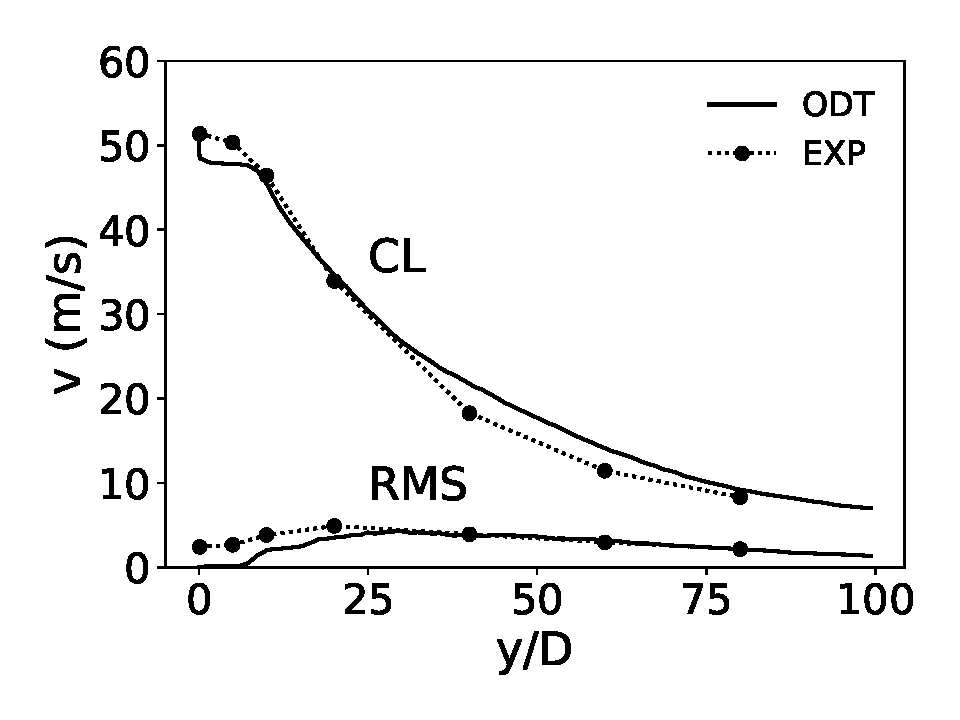
\includegraphics[width=1.7in]{../figures/cl_uvel_DLR_test_11.pdf} &
			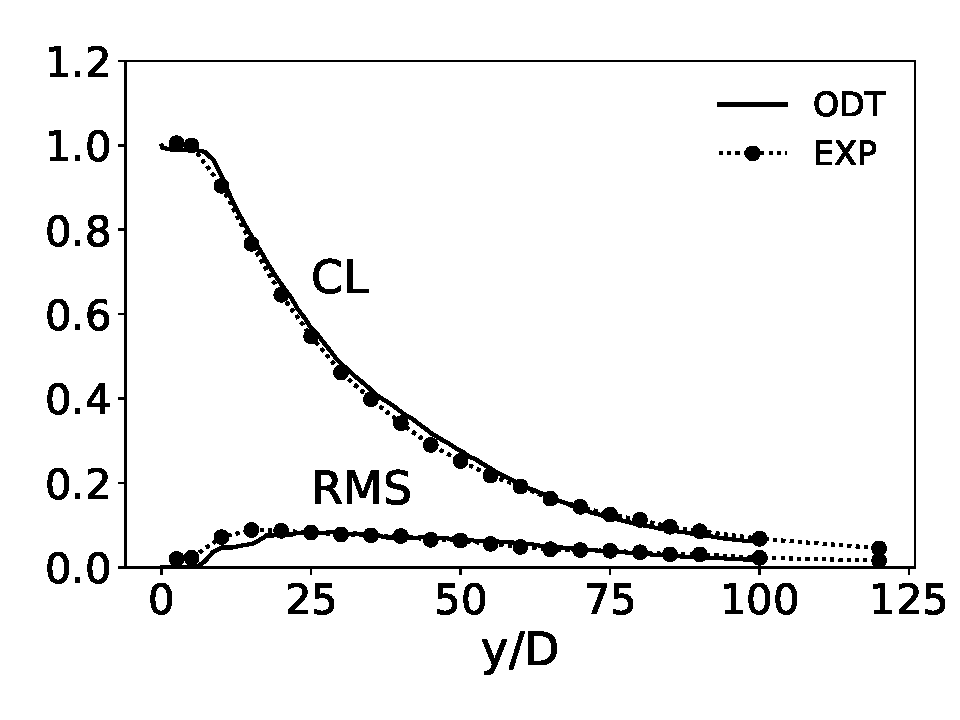
\includegraphics[width=1.7in]{../figures/cl_mixf_DLR_test_11.pdf} &
			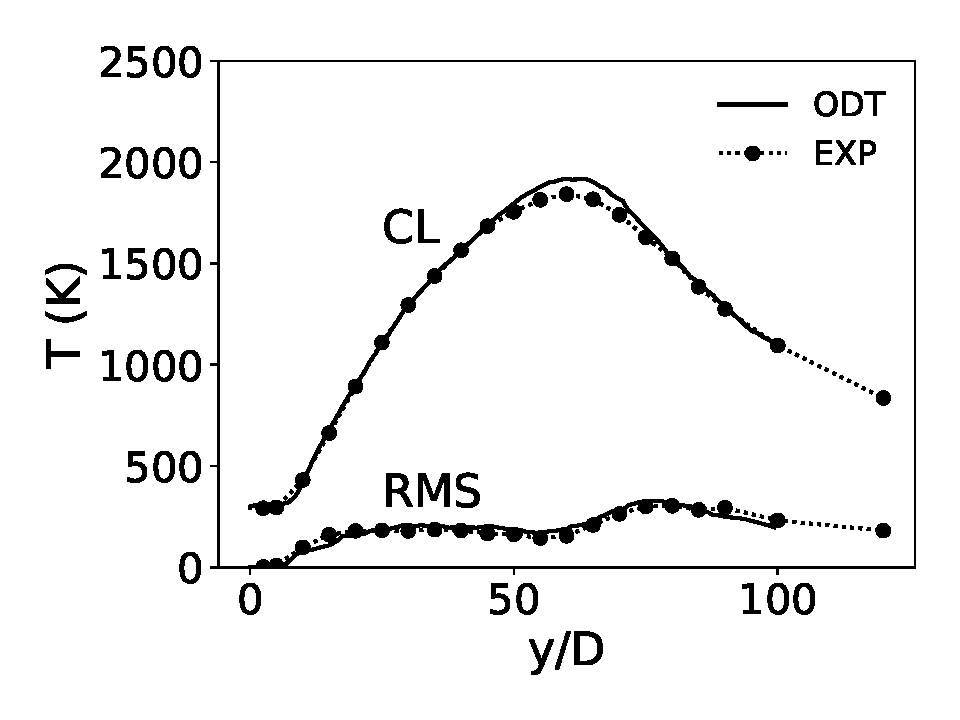
\includegraphics[width=1.7in]{../figures/cl_temp_DLR_test_11.pdf}
		\end{tabular}
	\end{center}
	\label{fig:dlr_example_results}
	\caption{DLR jet flame example case results: (a) mean axial velocity and RMS velocity along the centerline versus downstream location; (b) mean axial mixture fraction and RMS mixture fraction along the centerline versus downstream location; (c) mean axial temperature (K) and RMS temperature (K) along the centerline versus downstream location.}
\end{figure}

Figure~\ref{fig:dlr_example_results} displays the simulation results: axial mean and centerline values for (a) axial velocity $v$, (b) mixture fraction $\xi$, and (c) temperature $T$. The ODT results track the experimental data well for all three variables. The centerline temperature peaks about 100 K above the experimental data, but this small difference can be attributed to thermal radiation (which was neglected in this simulation) and the assumption that reactions proceed to the products of complete combustion rather than their equilibrium state. The centerline velocity shows a fast initial decrease that can be attributed to diffusion. Similarly, the increase in centerline velocity RMS values is delayed; this occurs due to the elapsed time model for large eddy suppression, which limits disturbances in the early stages of the flow to small eddies that occur on the jet edges away from the centerline. 

To replicate this example case, build the code with the \texttt{CHEMISTRY = SIMPLEDLR} flag in the \texttt{user\textunderscore config} file and edit the desired run script with \texttt{inputDir = "../input/jetFlame/DLR\textunderscore A"} and a new case name such as \texttt{caseName = "jetFlame\textunderscore example"}. The input file for this case, located at \texttt{ODT/input/jetFlame/DLR\textunderscore A/input.yaml}, contains the appropriate parameters and does not need to be modified to match this example case. See the code documentation for data post-processing instructions.

%Present the major functionalities of the software. 
%\begin{itemize}
%	\item simulating turbulent flow cases, reacting or nonreacting flows
%	\item can simulate laminar flow cases too
%	\item does these things a whole lot faster than other methods do (LES, DNS especially)
%	\item testing LES subgrid modeling assumptions
%	\item simulating cases that DNS can't get to because needed simulation length is too long (i.e. late-flame phenomena)
%\end{itemize}

%%%%%%%%%%%%%%%%%%%%%%%%%%%%%%%%%%%%%%%%%%%%%%%%%%%%%%%%%%%%%%%%%%%%%%%%%%%%%%%
\section{Impact}
\label{sec:impact}

Questions to answer in this section (from SoftwareX template)
\begin{enumerate}
	\item How can new research questions be pursued with this software?
		\begin{itemize}
			\item possibility of parametric studies (much harder with DNS/LES/RANS)
			\item study of late-flame soot and radiation interactions, soot emissions as smoke
			\item comparative radiation model studies?
		\end{itemize}
	\item How does the software improve pursuit of existing research questions?
		\begin{itemize}
			\item late-flame behavior becomes easier to study
			\item validation of LES subgrid models
			\item soot stuff, especially late in the flame (because soot moves slowly compared to gas species and therefore short simulation times like in DNS aren't enough to study it effectively)
		\end{itemize}
	\item How does the software change the daily practice of its users?
		\begin{itemize}
			\item cases take hours or days rather than weeks using supercomputer resources
			\item test cases can be run on local computers (unlike something like DNS) and as background tasks without disrupting other tasks
			\item ODT as a tool complements other approaches, can cover blind spots and be used in validation
		\end{itemize}
	\item How widespread is the software? Who uses it? (Within and outside of intended research area and/or group.)
		\begin{itemize}
			\item BYU group
			\item JCH at Sandia
			\item Chalmers group in Sweden (Marco Fistler, etc.)
			\item German university group (Heiko Schmidt, Juan Media, Marten Klein, etc.)
			\item TO DO: find other groups who have used or currently use ODT
		\end{itemize}
	\item How is the software used in commercial settings (if any)? Has it led to creation of spin-off companies?
		\begin{itemize}
			\item No commercial use (I think). 
		\end{itemize}
\end{enumerate}

%%%%%%%%%%%%%%%%%%%%%%%%%%%%%%%%%%%%%%%%%%%%%%%%%%%%%%%%%%%%%%%%%%%%%%%%%%%%%%%
\section{Conclusion}
\label{sec:conclusion}

Write this part next to last
%Set out the conclusion of this original software publication.

%%%%%%%%%%%%%%%%%%%%%%%%%%%%%%%%%%%%%%%%%%%%%%%%%%%%%%%%%%%%%%%%%%%%%%%%%%%%%%%
\section{Conflict of Interest}
%Please select the appropriate text:
%
%Potential conflict of interest exists:
%We wish to draw the attention of the Editor to the following facts, which may be considered as potential conflicts of interest, and to significant financial contributions to this work. The nature of potential conflict of interest is described below: [Describe conflict of interest]

%No conflict of interest exists:
There are no known conflicts of interest associated with this publication and there has been no significant financial support for this work that could have influenced its outcome.

%%%%%%%%%%%%%%%%%%%%%%%%%%%%%%%%%%%%%%%%%%%%%%%%%%%%%%%%%%%%%%%%%%%%%%%%%%%%%%%
\section*{Acknowledgements}
\label{acknoledgements}

This work was supported in part by the National Science Foundation under Grant No. CBET-1403403.

%Special thanks to Alan R. Kerstein for his significant contributions to model development. Additional thanks to Heiko Schmidt, Juan Medina, and Marten Klein of Brandenburg University of Technology Cottbus-Senftenberg, Michael Oevermann and Marco Fistler of Chalmers University of Technology, and Vladimir P. Solovjov of Brigham Young University.

%%%%%%%%%%%%%%%%%%%%%%%%%%%%%%%%%%%%%%%%%%%%%%%%%%%%%%%%%%%%%%%%%%%%%%%%%%%%%%%
%% The Appendices part is started with the command \appendix;
%% appendix sections are then done as normal sections
%% \appendix

%% \section{}
%% \label{}

%%%%%%%%%%%%%%%%%%%%%%%%%%%%%%%%%%%%%%%%%%%%%%%%%%%%%%%%%%%%%%%%%%%%%%%%%%%%%%%
%% References:

\bibliographystyle{elsarticle-num} 
\bibliography{references} 

%%%%%%%%%%%%%%%%%%%%%%%%%%%%%%%%%%%%%%%%%%%%%%%%%%%%%%%%%%%%%%%%%%%%%%%%%%%%%%%
\section*{Current executable software version}
\label{software_version}

Software information is provided in Table~\ref{t:software}.

%Ancillary data table required for sub version of the executable software: (x.1, x.2 etc.) kindly replace examples in right column with the correct information about your executables, and leave the left column as it is.

\begin{table}[!h]
\begin{tabular}{|l|p{6.5cm}|p{6.5cm}|}
\hline
\textbf{Nr.} & \textbf{(Executable) software metadata description} & \textbf{Please fill in this column} \\
\hline
S1 & Current software version & 1.0 \\
\hline
S2 & Permanent link to executables of this version  & For example: \href{https://github.com/BYUignite/ODT}{https://github.com/BYUignite/ODT} \\
\hline
S3 & Legal Software License & MIT \\
\hline
S4 & Computing platforms/Operating Systems & Linux, OS X, Microsoft Windows\\
\hline
S5 & Installation requirements \& dependencies & CMake 3.12+, Cantera, Git, Doxygen (optional) \\
\hline
S6 & If available, link to user manual - if formally published include a reference to the publication in the reference list & \href{https://byuignite.github.io/ODT/doxygen/html/index.html}{https://byuignite.github.io/ODT/doxygen/html/index.html}\\
\hline
S7 & Support email for questions & davidlignell@byu.edu \\
\hline
\end{tabular}
\caption{Software metadata (optional)}
\label{t:software}
\end{table}

\end{document}
\endinput
